We assume that the stellar density profile follows a broken power law
with the stellar density $\rhostar\sim r^{-1-\Gamma}= r^{-\delta}$ inside of the
break radius $\rb$, where ($0<\Gamma<1$). We derive an expression for
the specific enthalpy of the gas, $\ke +\gammaf \frac{p}{\rho}$ as a
function of $\zeta=v_w/\sigma$, $x=r/r_s$, and $r_s/\rsoi$. We show
that if the break radius, $\rb$ goes to infinity this quantity
necessarily goes to infinity as the potential well becomes infinitely
deep, hence a break radius is necessary for an outflow to be possible.

Consider the steady state energy conservation equation. {\bf AG perhaps
  put a brief explanation of how this relates to the steady state
  entropy equation via laws of thermodynamics?.}

\begin{align}
\frac{1}{r^2} \frac{d}{dr} \left(r^2 \rho v \left(\frac{v^2}{2} + \Phi
    + \gammaf \frac{p}{\rho}\right) \right) = q \kew + q \Phi
\label{eq:enCons}
\end{align}

Where $\kew=v_w^2+\sigma^2\simeq v_w^2+\frac{G M_{\rm enc}(r)}{r}$ and
$\Menc$ is the sum of the black hole mass and the stellar mass.

Now integrate both sides with respect from r to the stagnation radius 

\begin{align}
  r^2 \rho v \left(\ke+\Phi+\gammaf \frac{p}{\rho} \right)= \int_{\rs}^{r}
    r^2 \left(q \kew + q\Phi\right) dr
    \label{eq:enConsInt}
\end{align}

We know $f\equiv r^2 \rho v$ from the steady state mass conservation
equation. 

\begin{align}
 \frac{1}{r^2} \frac{d}{dr} \left(r^2 \rho v\right) = q 
\end{align}

Where q is the rate of the mass injection per volume, which is
proportional to the stellar density. Let $x=r/\rs$ and $q_o= q
(\rs)$. Then $q=q_o x^{-\delta}$. 

Then one obtains for the mass flux, $f$ 

\begin{align}
 f(x)=q_o \rs^3 \left[\frac{x^{3-\delta}-1}{3-\delta}\right]
 \label{eq:massFlux}
\end{align}

The gravitational potential $\Phi$ is given by

\begin{align}
\Phi= -\frac{G \Menc}{r} - 4 \pi G \int_{r}^{\rs} \rhostar(dr') r'
dr'.
\label{eq:Phi}
\end{align}

Note our unconventional choice of gauge: the upper limit of the
integral on the right hand side is $\rs$ whereas conventionally the
upper limit is taken to be $\infty$. This means that our definition
will not give $\Phi=0$ in the limit $r\rightarrow\infty$. However,
our result for the enthalpy $\ke + \gammaf \frac{p}{\rho}$ will be
gauge invariant. 

Using equations~\eqref{eq:enConsInt},~\eqref{eq:massFlux},
and~\eqref{eq:Phi}, we may obtain an expression for the enthalpy,
$\ke+\gammaf \frac{p}{\rho}$ of the gas inside of the break radius
$\rb$. 

\begin{align}
  &\frac{v^2}{2}+\gammaf \frac{p}{\rho} = \frac{G \Mbh}{x \rs} +
  \frac{G
    M_\star}{x \rs} - U_o \frac{x^{2-\delta}-1}{2-\delta}\nonumber\\
  &-U_o\left[\frac{1}{2-\delta}-\frac{x^{5-2\delta}-1}{x^{3-\delta}-1}\frac{3-\delta}{(5-2\delta)(2-\delta)}\right]\nonumber\\
  &+\frac{v_w^2}{2}+\frac{\sigma_0^2}{2}- \frac{G \Mbh}{r_s}
  \frac{1-2\delta}{2(\delta+1)} \frac{3-\delta}{2-\delta}\frac{x^{2-\delta}-1}{x^{3-\delta}-1}
  \nonumber\\
  &-\frac{G M_\star}{r_s}
  \frac{x^{5-2\delta}-1}{x^{3-\delta}-1}\frac{3-\delta}{5-2\delta},
\end{align}

where $U_o=4 \pi G \rhostar(\rs) \rs^2$.  We may rewrite this as 

\begin{multline}
  \frac{v^2}{2}+\gammaf \frac{p}{\rho}
=\frac{G \Mbh}{\rs} 
\biggl[
  \frac{3}{2} \zeta^2 w^{\frac{1}{3 -\delta}}+\frac{1}{x}+\frac{w}{x}
  -\frac{(1-2\delta)(3-\delta)}{2(\delta+1)(2-\delta)}  \frac{x^{2  -\delta}-1}{x^{3-\delta}-1}\\
  -w \frac{3 -\delta}{2 -\delta} x^{2 -\delta}
  -w \frac{(2-\delta)(3-\delta)-(3-\delta)^{2}}{(5-2\delta)(2-\delta)} \frac{x^{5-2\delta}-1}{x^{3-\delta}-1}
\biggr].
\label{eq:enthAnal}
\end{multline}

Recall that $\rs$ the stagnation radius, $x\equiv r/\rs$, $\zeta=\sqrt{(v_w^2+\sigma_0^2)/\sigma_0}$, $w\equiv (\rs/\rsoi)^{3\delta}$, and
$\delta$ is the power law slope of the stellar density profile inside
of the break radius, $\rb$.

For a given $\zeta$ we define a critical $\rs/\rsoi=min{
  \frac{frac{7}{2}-\densSlope}{\densSlope \zeta^2, 1}}$ for thermal stability, 
where the first term in the brackets corresponds to twice the value
predicted by equation~\eqref{eq:rsRinf}, in the limit the stellar mass
as $\rs$ is small compared to $\Mbh$. This prescription is somehwat
ad hoc, but...{\bf AG--some motivation...}

Then from equation~\eqref{eq:enthAnal} we may obtain the critical
wind heating parameter $v_{w, \rm crit}/\sigma_{\rm inf}$ for thermal stability as
a function of $\rb/\rsoi$. This is shown in Fig.~\ref{fig:vwCrit}

\begin{figure}
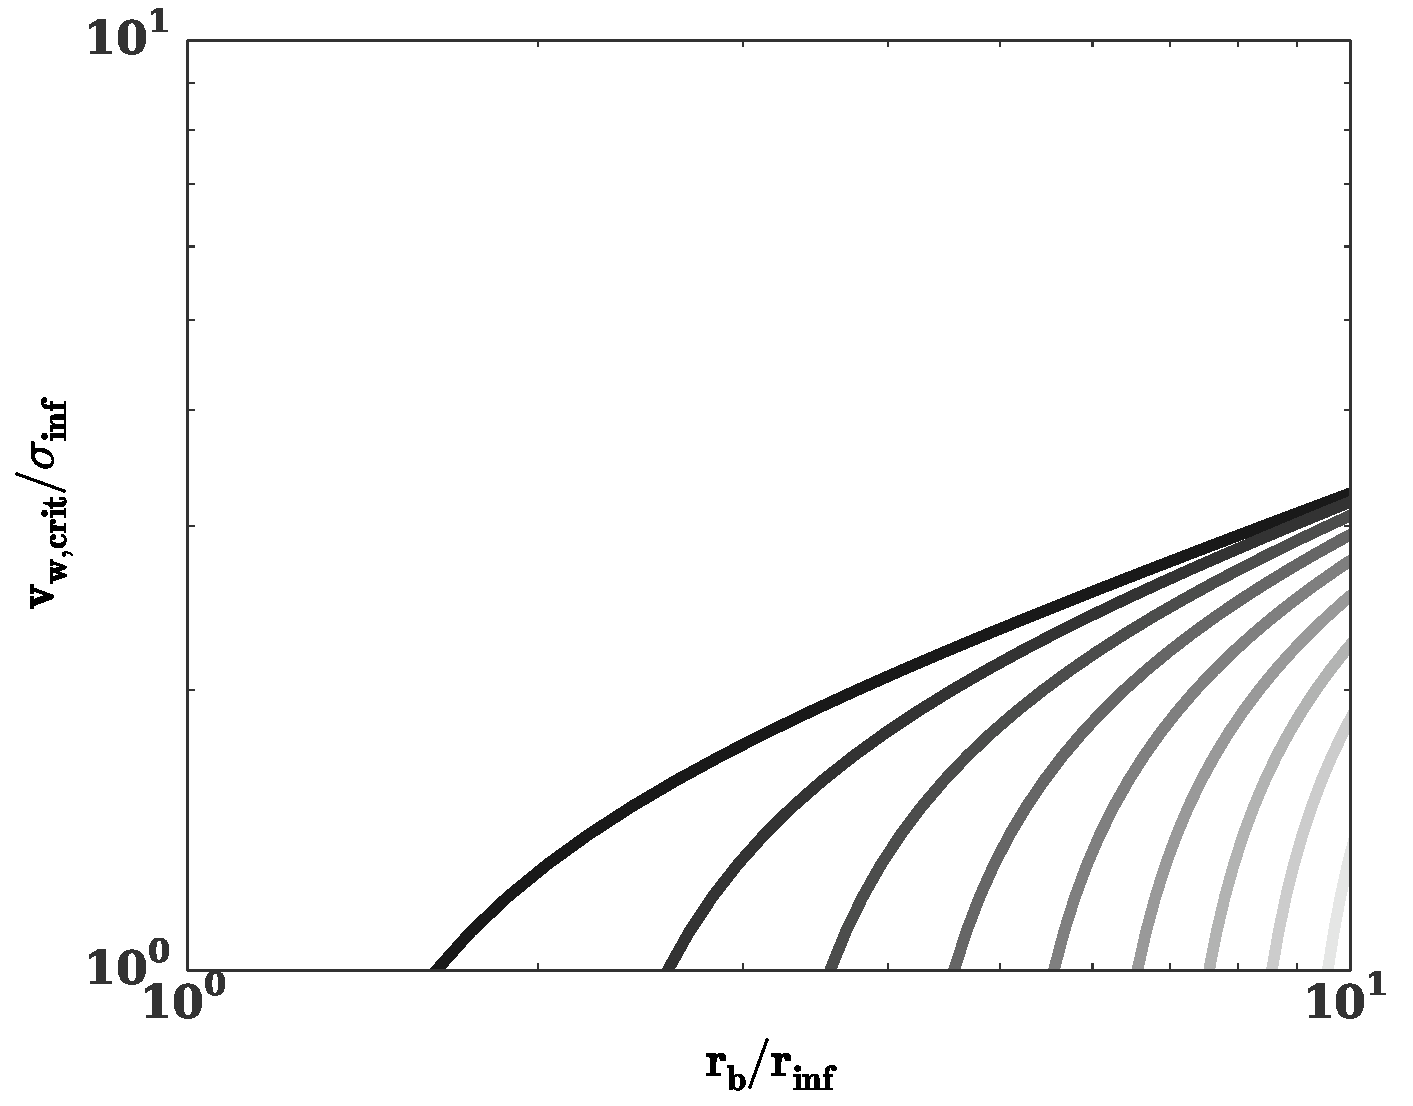
\includegraphics[width=\columnwidth]{vwCrit.pdf}
\caption{\label{fig:vwCrit} Critical heating rate required for thermal
  stability normalized to the velocity dispersion at the sphere
  influence radius, $\sigma_{\rm soi}$ versus $\rb/\rsoi$, the ratio
  of the break radius in the stellar density profile to the sphere of
  influence radius. We assume a core stellar dnsity profile inside of
  $\rb$, so that $\rhostar\sim r^{-1-\Gamma}$ with $\Gamma=0.1$.}
\end{figure}


%%% Local Variables: 
%%% mode: latex
%%% TeX-master: "ms"
%%% End: 
